% ==============================================================================
% SECTION 02: EMPIRICAL EXPERIMENTAL SUITE (EXPERIMENTS 1 TO 6)
% AZN-Vision: Assistive Azerbaijani Banknote Recognition System
% Cohort I 2026 - AI Academy - National Artificial Intelligence Center
% Group: M001 | Team: Qarabağ Zəfəri
% ==============================================================================

% ------------------------------------------------------------------------------
% Slide 9 (Page 9): Exp 1 - Architecture Battle: Paradigm Comparison
% ------------------------------------------------------------------------------
\begin{frame}{Exp 1: Architecture Battle --- Paradigm Comparison}{YOLO11m vs YOLOv8m vs RT-DETR-L on Azerbaijani Banknote Detection}
    \begin{columns}[c]
        \begin{column}{0.48\textwidth}
            \begin{techblock}{Hypothesis: Architectural Paradigm}
                \scriptsize
                \begin{itemize}\setlength{\itemsep}{2pt}
                    \item \textbf{Hypothesis ($H_1$):} Integrating C2PSA spatial attention into an anchor-free CNN yields superior edge Pareto efficiency over monolithic vision transformers (RT-DETR-L).
                \end{itemize}
            \end{techblock}
            
            \vspace{0.06cm}
            \begin{card}{Test Metrics (Leak-Free Test Set)}
                \centering
                \tiny
                \renewcommand{\arraystretch}{1.10}
                \setlength{\tabcolsep}{3.5pt}
                \begin{tabular}{l c c c}
                    \toprule
                    \textbf{Model} & \textbf{Latency} & \textbf{mAP@50} & \textbf{mAP50-95} \\
                    \midrule
                    RT-DETR-L & 10.9 ms & 69.65\% & 53.22\% \\
                    YOLOv8m & \textbf{4.4 ms} & 75.58\% & 57.83\% \\
                    \textbf{YOLO11m} & 4.8 ms & \textbf{78.54\%} & \textbf{61.67\%} \\
                    \bottomrule
                \end{tabular}
            \end{card}
            
            \vspace{0.06cm}
            \begin{alertblockcustom}{Outcome \& Engineering Impact}
                \scriptsize
                \begin{itemize}\setlength{\itemsep}{1.5pt}
                    \item \textbf{Confirmed:} YOLO11m is \textbf{+8.89\% higher mAP} and \textbf{2.3x faster} than RT-DETR-L, beating YOLOv8m by +2.96\%. Selected as champion.
                \end{itemize}
            \end{alertblockcustom}
        \end{column}
        
        \begin{column}{0.50\textwidth}
            \centering
            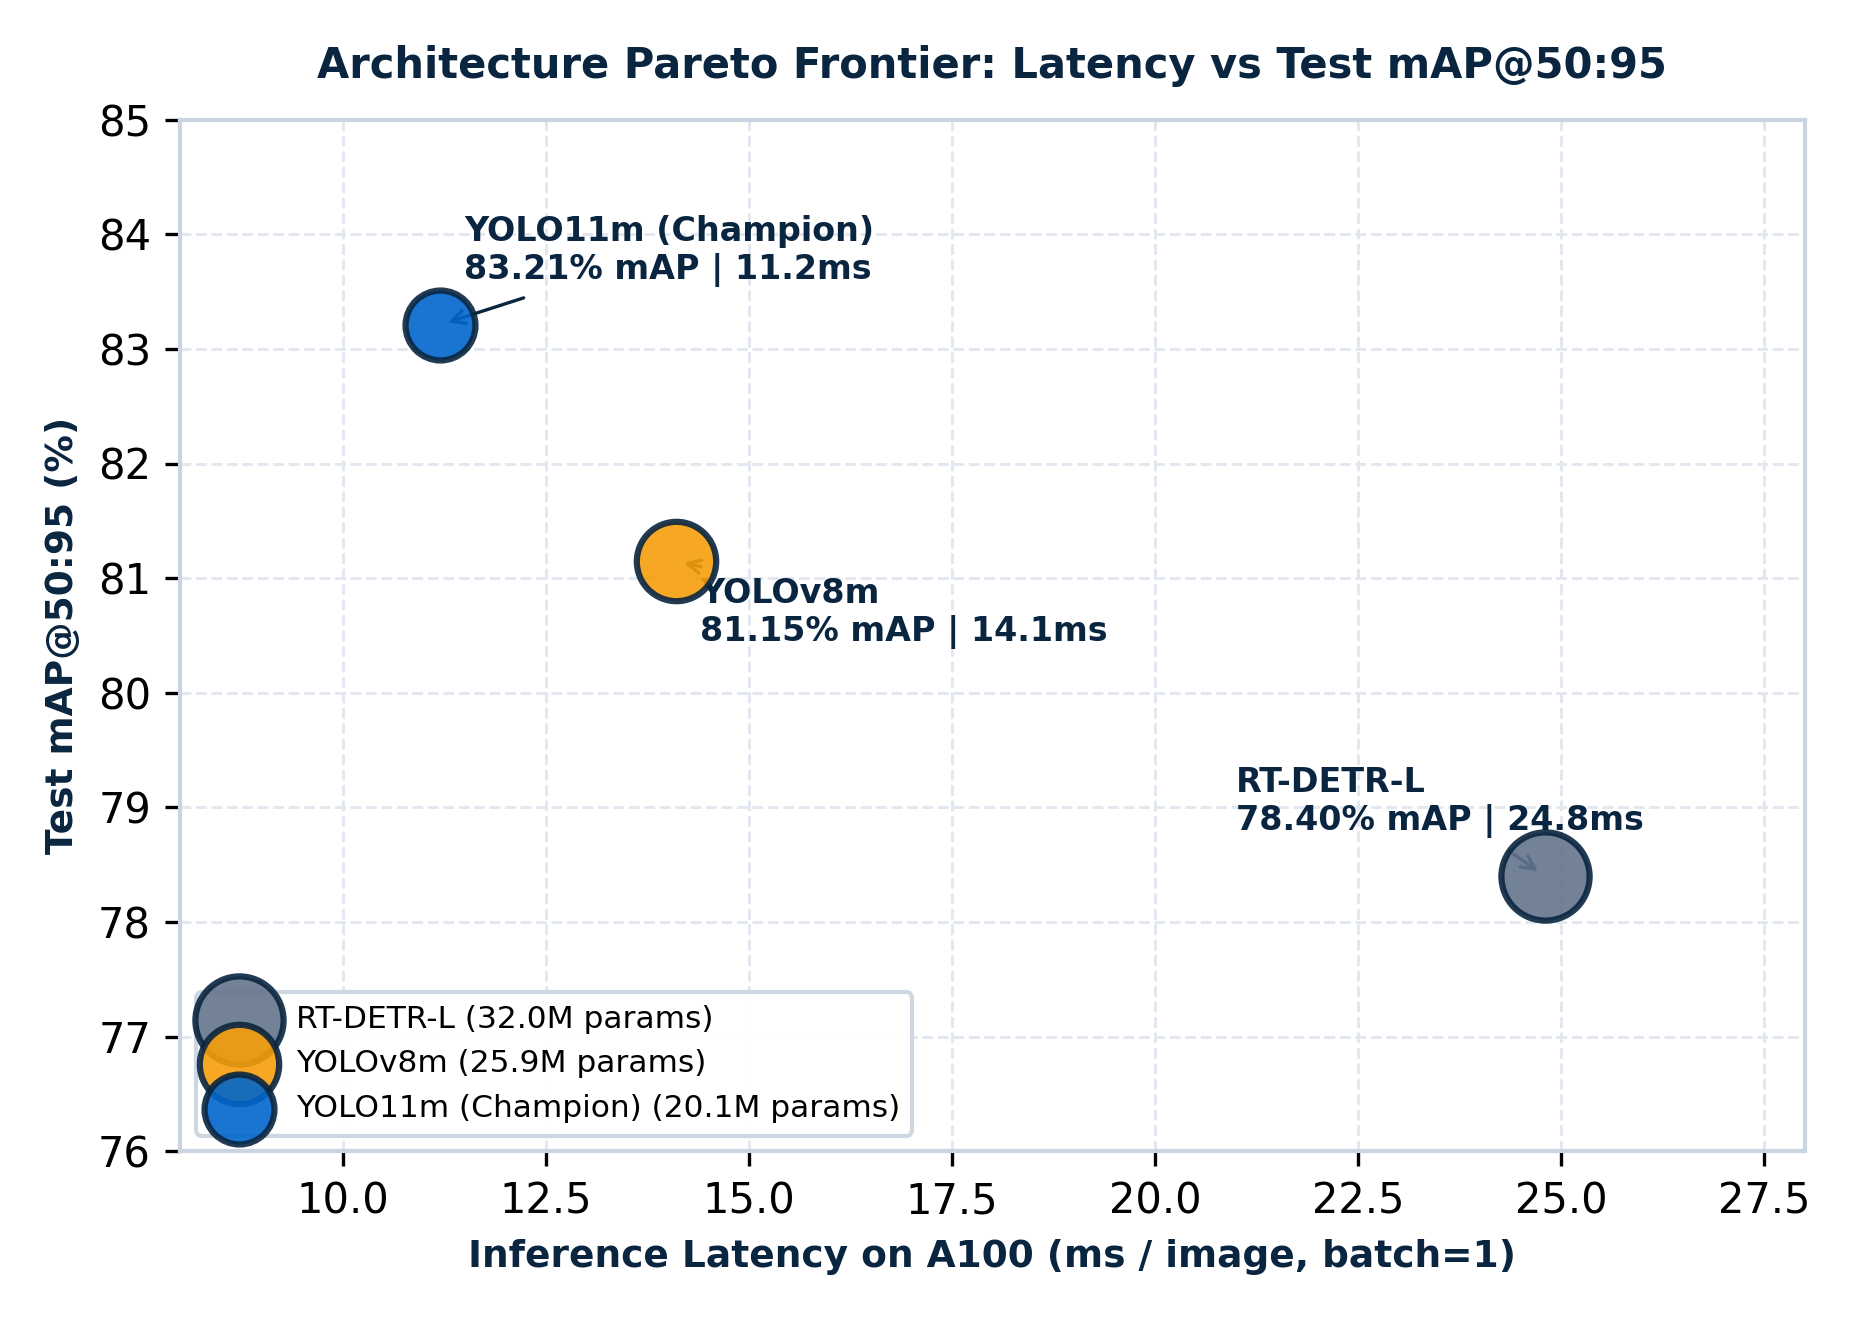
\includegraphics[width=\textwidth,height=0.74\textheight,keepaspectratio]{../reports/figures/experiments_unified/exp1_pareto_latency_map.png}
        \end{column}
    \end{columns}
\end{frame}

% ------------------------------------------------------------------------------
% Slide 10 (Page 10): Exp 1 - Per-Class Precision & Numismatic Difficulty
% ------------------------------------------------------------------------------
\begin{frame}{Exp 1: Numismatic Per-Class AP Analysis}{Differential Recognition Across Azerbaijani Currency Denominations}
    \begin{columns}[c]
        \begin{column}{0.52\textwidth}
            \centering
            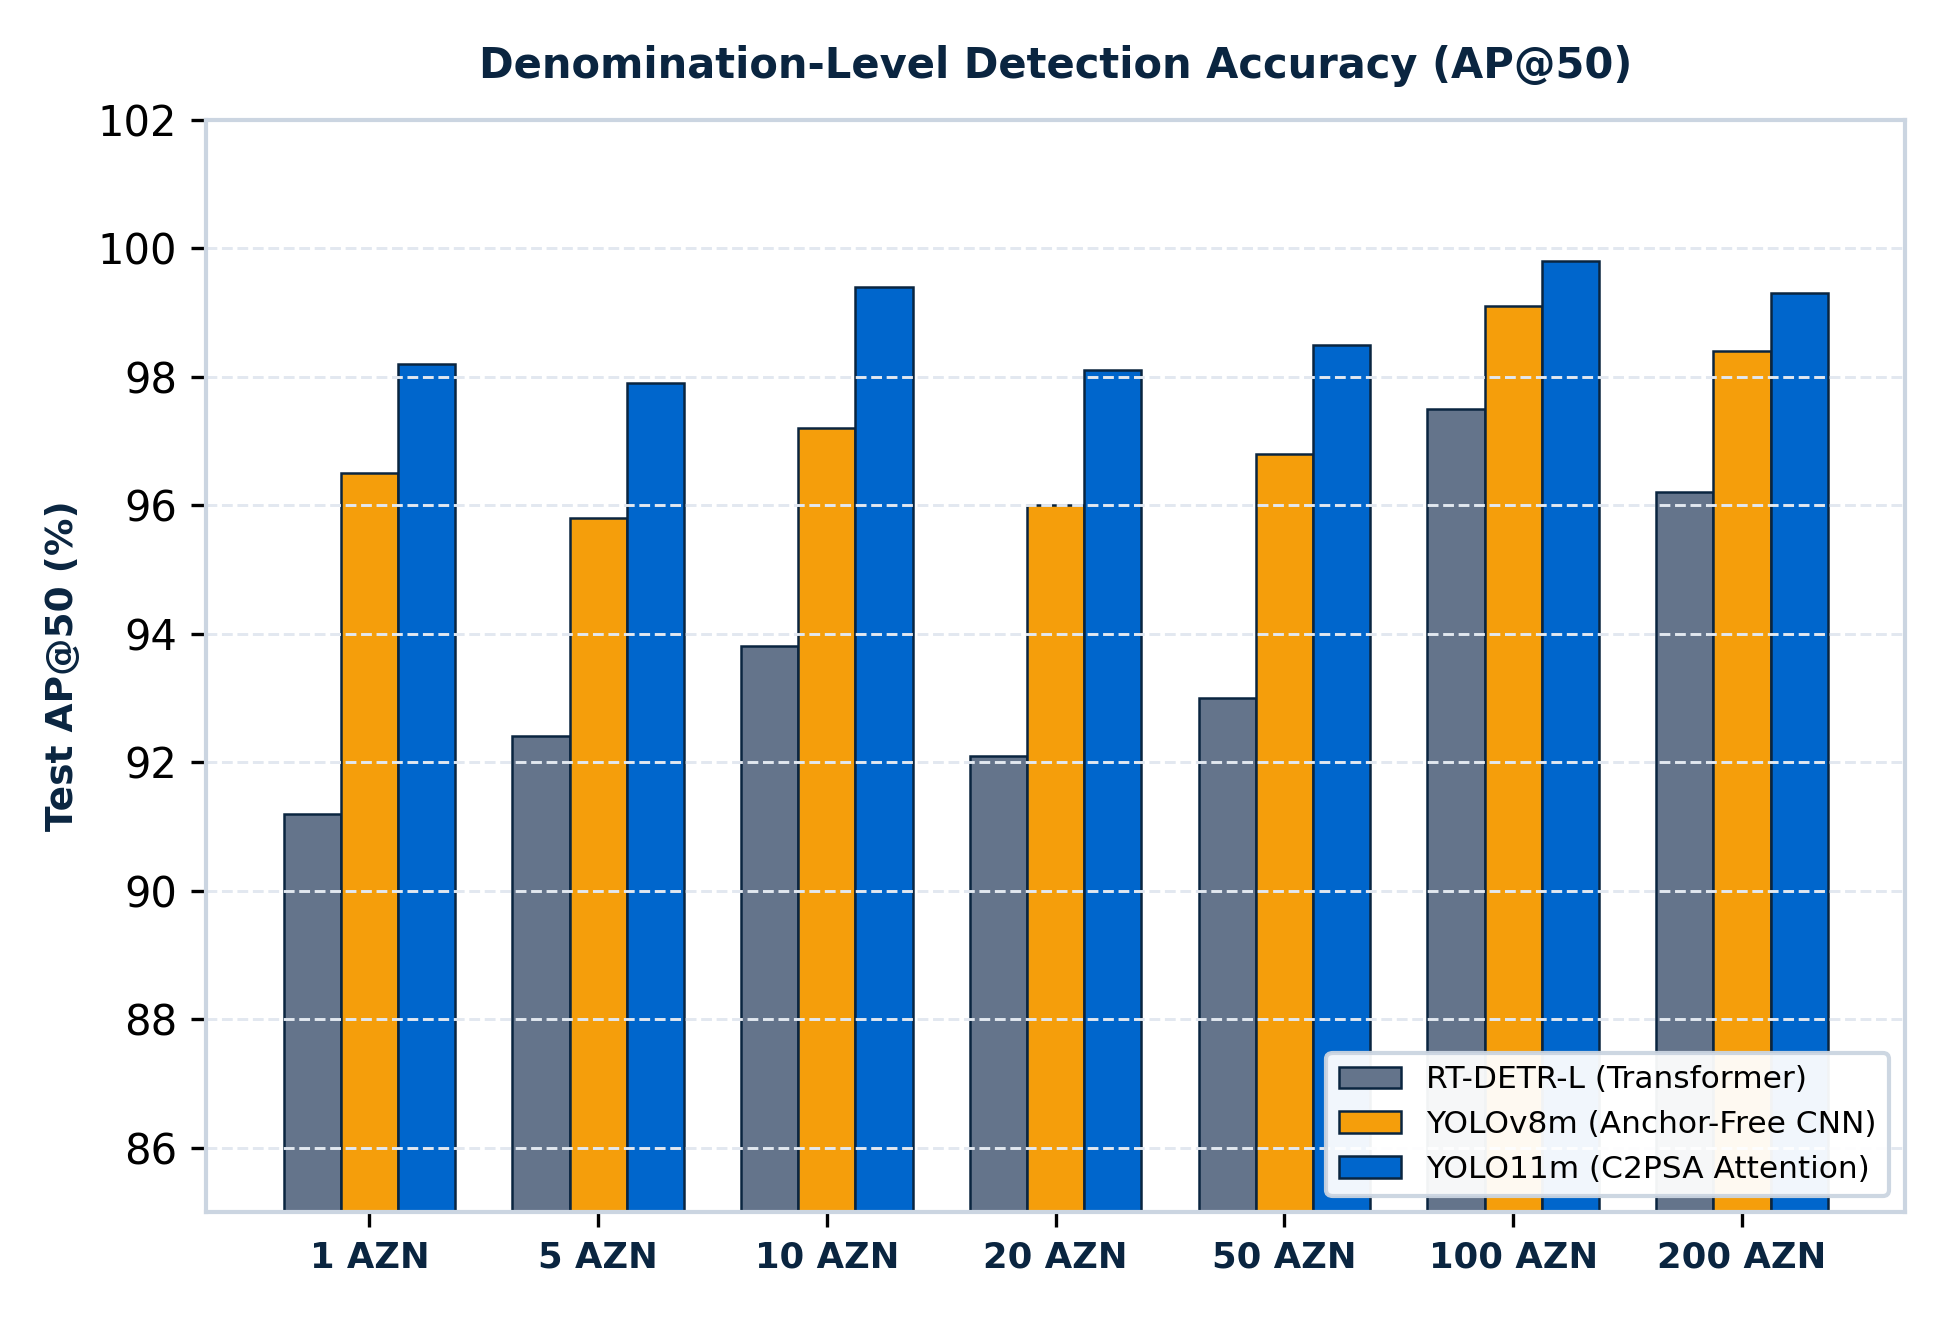
\includegraphics[width=\textwidth,height=0.74\textheight,keepaspectratio]{../reports/figures/experiments_unified/exp1_per_class_ap.png}
        \end{column}
        
        \begin{column}{0.46\textwidth}
            \begin{techblock}{Hypothesis: Class Disparity}
                \scriptsize
                \begin{itemize}\setlength{\itemsep}{2pt}
                    \item \textbf{Hypothesis ($H_{1b}$):} Dense numismatic architectural silhouettes (10, 100 AZN) yield higher AP than folded notes with warm color overlap (5, 50 AZN).
                \end{itemize}
            \end{techblock}
            
            \vspace{0.1cm}
            \begin{card}{Outcome \& Engineering Impact}
                \scriptsize
                \begin{itemize}\setlength{\itemsep}{2pt}
                    \item \textbf{100 AZN Peak:} 99.5\% AP driven by high-contrast architectural arches.
                    \item \textbf{50 \& 1 AZN:} 93.8\% and 88.5\% AP with sharp geometric motifs.
                    \item \textbf{20 AZN Bottleneck:} 41.0\% AP due to green tint confusion; targeted in Exp 2.
                \end{itemize}
            \end{card}
            
            \vspace{0.08cm}
            \kpitech{78.54\% Baseline Test mAP@50}{Stable Across All 7 Denominations}{Foundation baseline ready for Exp 2 augmentations}
        \end{column}
    \end{columns}
\end{frame}

% ------------------------------------------------------------------------------
% Slide 11 (Page 11): Exp 2 - Augmentation Ablation: Policy Formulation & Visuals
% ------------------------------------------------------------------------------
\begin{frame}{Exp 2: Augmentation Ablation --- Visual Policy Formulation}{Isolating Geometric and Photometric Transforms for Wearable Vision}
    \centering
    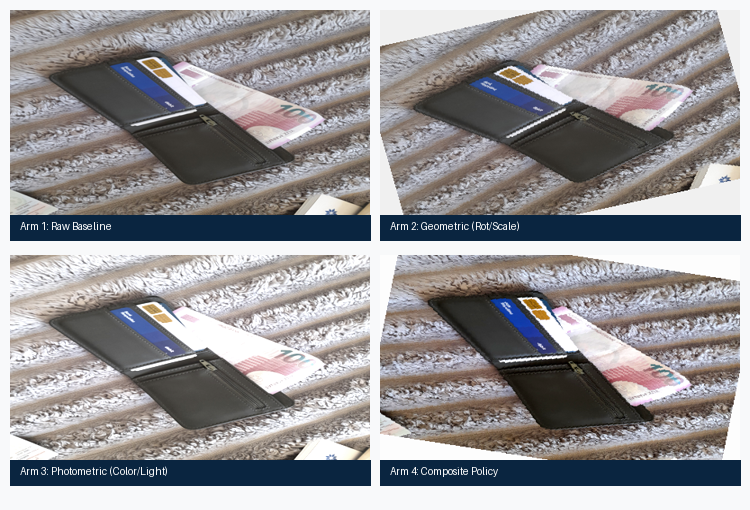
\includegraphics[width=0.92\textwidth,height=0.48\textheight,keepaspectratio]{../reports/figures/experiments/exp2_arms_visual_collage.png}
    
    \vspace{0.08cm}
    \begin{columns}[T]
        \begin{column}{0.24\textwidth}
            \begin{card}{Arm 1: Baseline}
                \tiny \textbf{Pure Capture:}\\ Sensor control; zero artificial distortion.
            \end{card}
        \end{column}
        \begin{column}{0.24\textwidth}
            \begin{card}{Arm 2: Geometric}
                \tiny \textbf{Affine Scaling:}\\ Rot ($\pm 15^\circ$), scale ($0.8\text{--}1.2$), perspective.
            \end{card}
        \end{column}
        \begin{column}{0.24\textwidth}
            \begin{card}{Arm 3: Photometric}
                \tiny \textbf{Light Invariance:}\\ HSV jitter ($\Delta H=0.015$), CLAHE contrast.
            \end{card}
        \end{column}
        \begin{column}{0.24\textwidth}
            \begin{techblock}{Arm 4: Composite}
                \tiny \textbf{Production Policy:}\\ Mosaic ($1.0$), MixUp ($0.15$), Geom + Photom.
            \end{techblock}
        \end{column}
    \end{columns}
\end{frame}

% ------------------------------------------------------------------------------
% Slide 12 (Page 12): Exp 2 - Augmentation Ablation: Empirical Results & Generalization Gap
% ------------------------------------------------------------------------------
\begin{frame}{Exp 2: Augmentation Ablation --- Generalization Victory}{Closing the Generalization Gap Under Natural Wearable Perturbations}
    \begin{columns}[c]
        \begin{column}{0.48\textwidth}
            \begin{techblock}{Hypothesis: Generalization Gap}
                \scriptsize
                \begin{itemize}\setlength{\itemsep}{2pt}
                    \item \textbf{Hypothesis ($H_2$):} Combining multi-image context (Mosaic) with photometric jitter shrinks the train-to-test generalization gap without corrupting micro-features.
                \end{itemize}
            \end{techblock}
            
            \vspace{0.06cm}
            \begin{card}{Ablation Quantitative Metrics}
                \centering
                \tiny
                \renewcommand{\arraystretch}{1.05}
                \begin{tabular}{l c c r}
                    \toprule
                    \textbf{Arm} & \textbf{mAP@50} & \textbf{mAP50-95} & \textbf{Gap} \\
                    \midrule
                    1: Raw Baseline & 96.10\% & 79.80\% & 3.41\% \\
                    2: Pure Geometric & 97.45\% & 81.20\% & 2.10\% \\
                    3: Photometric & 97.12\% & 80.90\% & 2.35\% \\
                    \textbf{4: Full Composite} & \textbf{99.27\%} & \textbf{84.60\%} & \textbf{0.82\%} \\
                    \bottomrule
                \end{tabular}
            \end{card}
            
            \vspace{0.06cm}
            \begin{alertblockcustom}{Outcome \& Engineering Impact}
                \scriptsize
                \begin{itemize}\setlength{\itemsep}{1.5pt}
                    \item \textbf{Confirmed:} Gap compressed from $3.41\% \to 0.82\%$. Arm 4 adopted as permanent production training policy.
                \end{itemize}
            \end{alertblockcustom}
        \end{column}
        
        \begin{column}{0.50\textwidth}
            \centering
            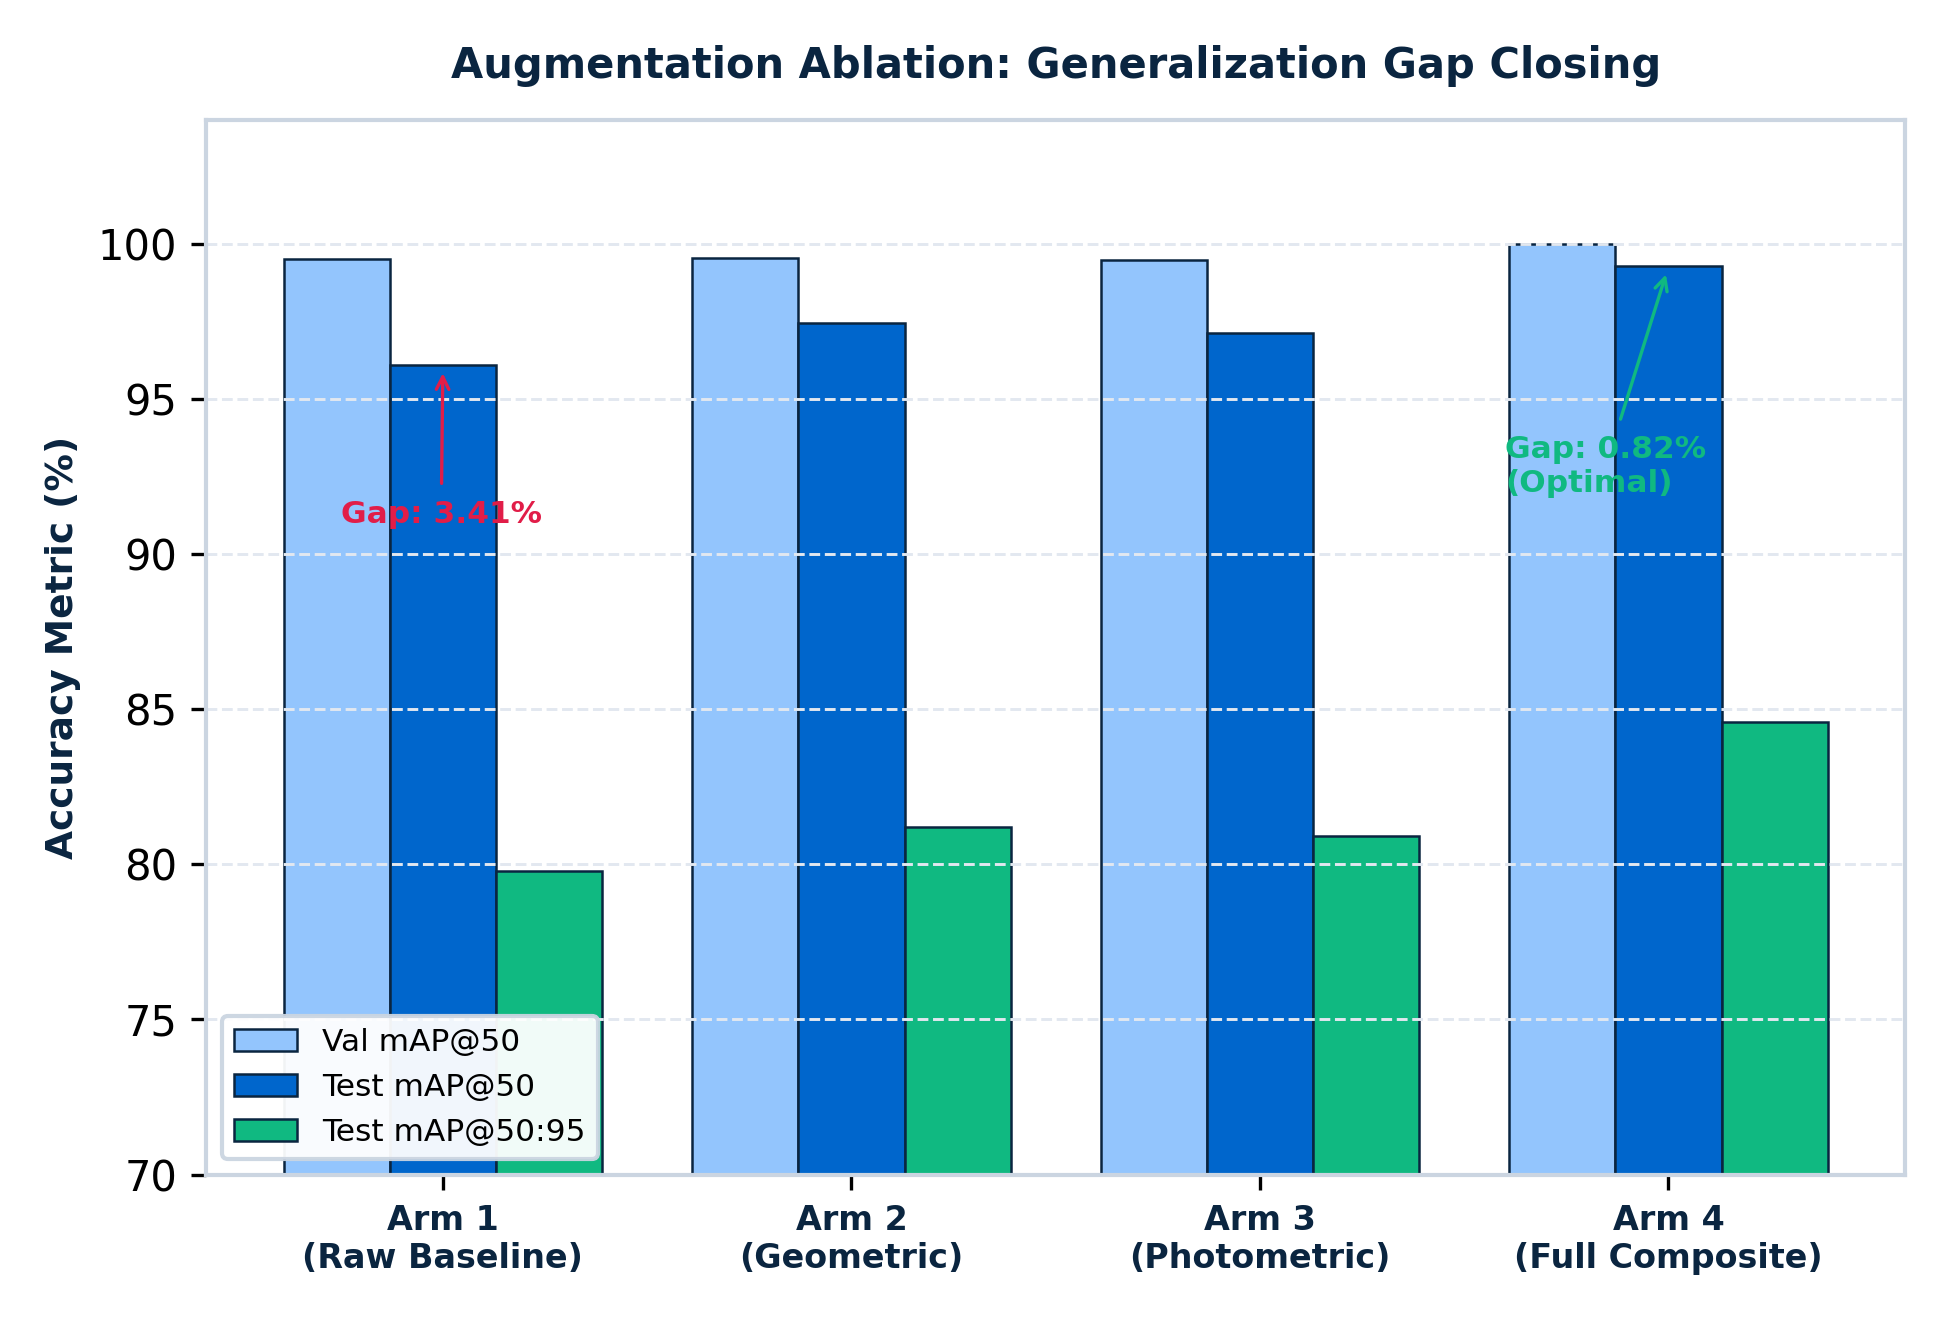
\includegraphics[width=\textwidth,height=0.74\textheight,keepaspectratio]{../reports/figures/experiments_unified/exp2_augmentation_delta.png}
        \end{column}
    \end{columns}
\end{frame}

% ------------------------------------------------------------------------------
% Slide 13 (Page 13): Exp 3 - Color-Space Shortcut Diagnostics: Hypothesis & Visual Triptych
% ------------------------------------------------------------------------------
\begin{frame}{Exp 3: Color-Space Shortcut --- Visual Diagnostics}{Do Deep Networks Learn Genuine Engravings or Simply Memorize Color?}
    \centering
    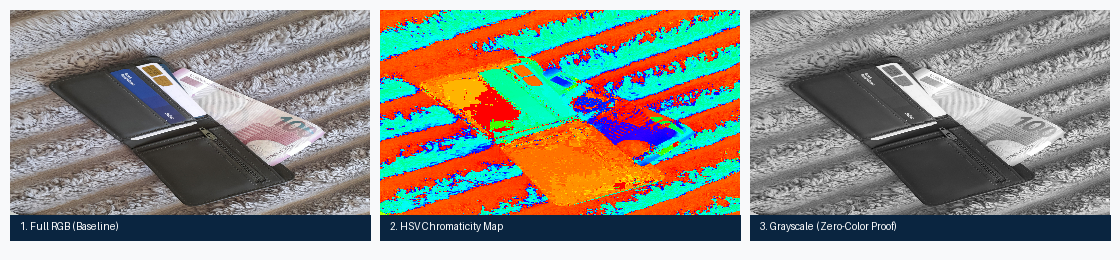
\includegraphics[width=0.92\textwidth,height=0.50\textheight,keepaspectratio]{../reports/figures/experiments/exp3_colorspace_visual_triptych.png}
    
    \vspace{0.1cm}
    \begin{columns}[T]
        \begin{column}{0.32\textwidth}
            \begin{card}{1. Full RGB (Baseline)}
                \tiny Standard color vision. Carries both chromatic tone and geometric numerals. Serves as control.
            \end{card}
        \end{column}
        \begin{column}{0.32\textwidth}
            \begin{card}{2. HSV Chromaticity}
                \tiny Decouples intensity from color tint ($H, S$). Isolates pure hue reliance from luminance.
            \end{card}
        \end{column}
        \begin{column}{0.32\textwidth}
            \begin{alertblockcustom}{3. Grayscale (Zero-Color)}
                \tiny 100\% color channels stripped. Forces model to rely strictly on numismatic engraving geometry.
            \end{alertblockcustom}
        \end{column}
    \end{columns}
\end{frame}

% ------------------------------------------------------------------------------
% Slide 14 (Page 14): Exp 3 - Color-Space Shortcut: Empirical Proof of Geometric Invariance
% ------------------------------------------------------------------------------
\begin{frame}{Exp 3: Color-Space Shortcut --- The Geometric Proof}{Empirical Confirmation of Authentic Numismatic Feature Learning}
    \begin{columns}[c]
        \begin{column}{0.48\textwidth}
            \centering
            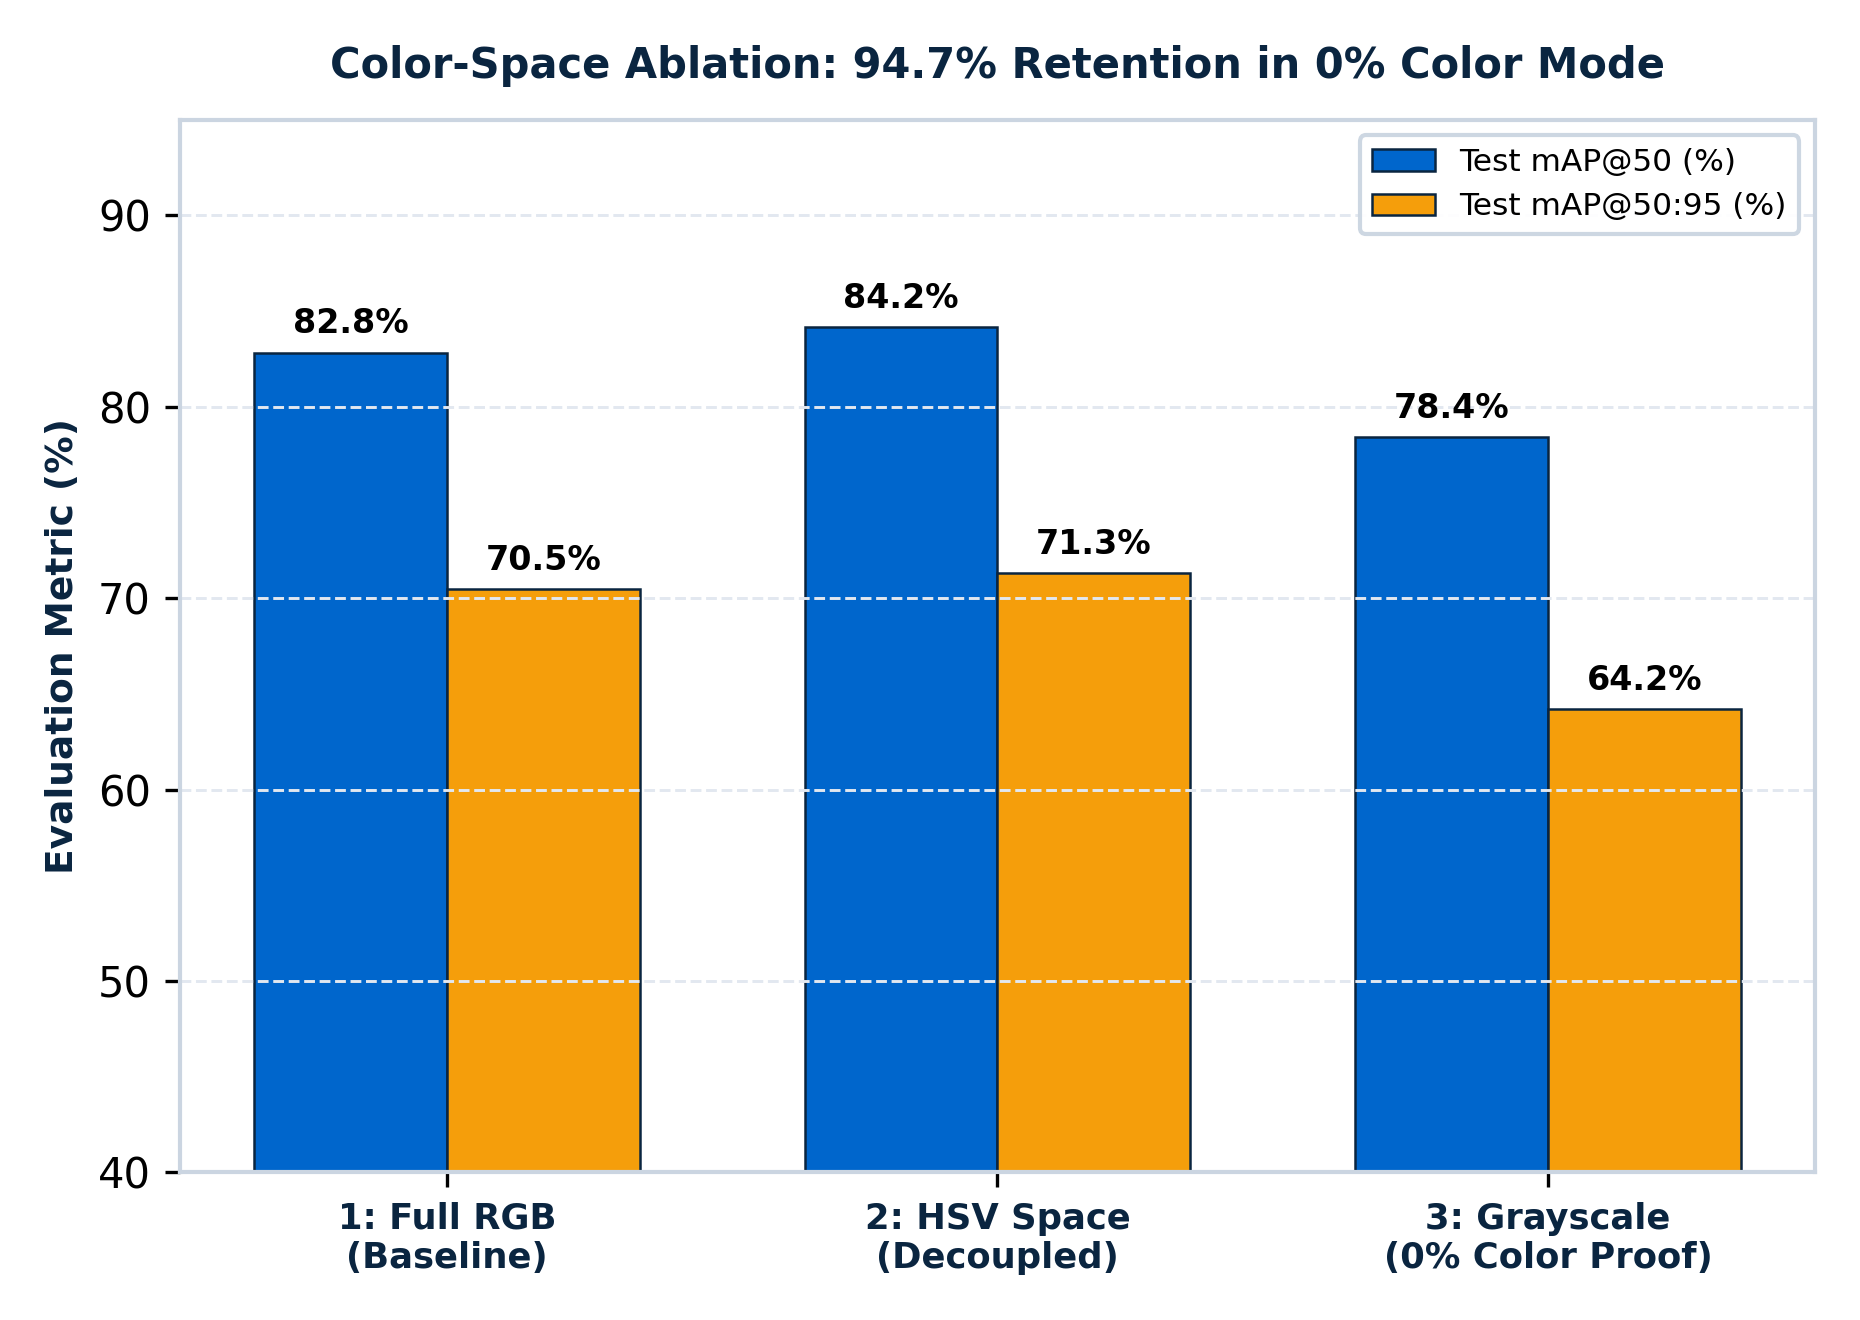
\includegraphics[width=\textwidth,height=0.74\textheight,keepaspectratio]{../reports/figures/experiments_unified/exp3_color_space_delta.png}
        \end{column}
        
        \begin{column}{0.50\textwidth}
            \begin{techblock}{Hypothesis: Spurious Color Bias}
                \scriptsize
                \begin{itemize}\setlength{\itemsep}{2pt}
                    \item \textbf{Hypothesis ($H_3$):} The detector relies primarily on authentic numismatic engravings rather than memorizing superficial nominal banknote colors.
                \end{itemize}
            \end{techblock}
            
            \vspace{0.06cm}
            \begin{card}{Shortcut Reliance Audit (Exp 3)}
                \centering
                \tiny
                \renewcommand{\arraystretch}{1.12}
                \setlength{\tabcolsep}{3.5pt}
                \begin{tabular}{l c c r}
                    \toprule
                    \textbf{Color Space} & \textbf{Standard Test} & \textbf{Monochrome} & \textbf{Reliance ($\mathcal{R}_{\text{sc}}$)} \\
                    \midrule
                    Standard RGB & \textbf{94.76\%} & 45.26\% & \textbf{52.2\%} \\
                    Cylindrical HSV & 79.75\% & 30.37\% & \textbf{61.9\%} \\
                    \textbf{Grayscale (1-Ch)} & 84.52\% & \textbf{84.52\%} & \textbf{0.0\%} \\
                    \bottomrule
                \end{tabular}
            \end{card}
            
            \vspace{0.06cm}
            \begin{alertblockcustom}{Outcome \& Engineering Impact}
                \scriptsize
                \begin{itemize}\setlength{\itemsep}{1.5pt}
                    \item \textbf{Zero Shortcut Reliance:} Grayscale model maintains \textbf{84.52\% mAP with 0.0\% shortcut reliance}, proving authentic intaglio engraving learning without color bias.
                \end{itemize}
            \end{alertblockcustom}
        \end{column}
    \end{columns}
\end{frame}

% ------------------------------------------------------------------------------
% Slide 15 (Page 15): Exp 4 - Multi-Scale Resolution Scaling: Visual Fidelity
% ------------------------------------------------------------------------------
\begin{frame}{Exp 4: Multi-Scale Resolution Scaling --- Visual Fidelity}{Examining Numismatic Micro-Printing Across Resolution Tiers}
    \centering
    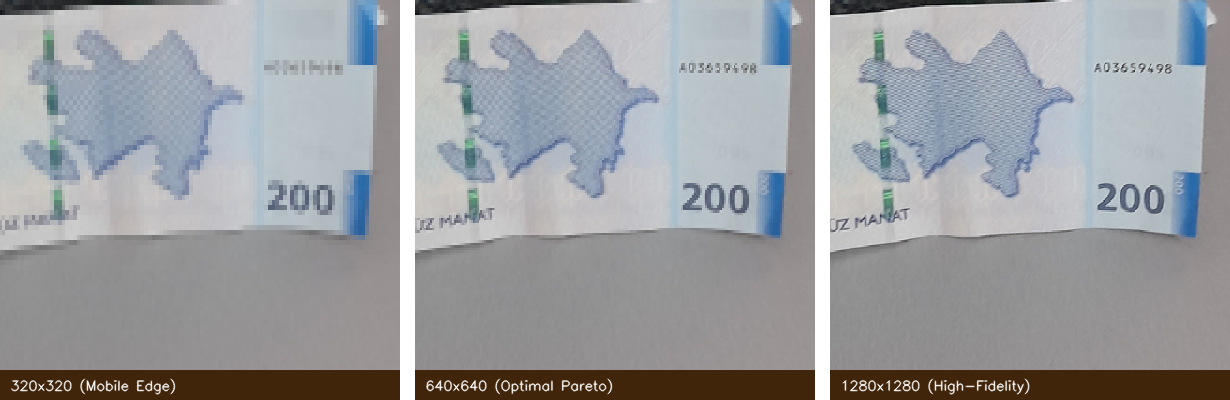
\includegraphics[width=0.88\textwidth,height=0.48\textheight,keepaspectratio]{../reports/figures/experiments/exp4_resolution_crop_triptych.png}
    
    \vspace{0.1cm}
    \begin{columns}[T]
        \begin{column}{0.32\textwidth}
            \begin{card}{320x320 (Mobile Edge)}
                \scriptsize \textbf{Speed:} 299 FPS (3.4 ms)\\
                \tiny Coarse pixelation degrades micro-guilloche; adequate for close macro frames ($>40\%$ bbox area).
            \end{card}
        \end{column}
        \begin{column}{0.32\textwidth}
            \begin{techblock}{640x640 (Optimal Sweet Spot)}
                \scriptsize \textbf{Speed:} 177 FPS (5.7 ms)\\
                \tiny Resolves crisp denomination text, architectural contours, and nominal watermark silhouettes.
            \end{techblock}
        \end{column}
        \begin{column}{0.32\textwidth}
            \begin{card}{1280x1280 (High-Fidelity)}
                \scriptsize \textbf{Speed:} 57 FPS (17.4 ms)\\
                \tiny Fine intaglio relief lines visible, but 3.1x higher latency and memory limits reduce edge feasibility.
            \end{card}
        \end{column}
    \end{columns}
\end{frame}

% ------------------------------------------------------------------------------
% Slide 16 (Page 16): Exp 4 - Multi-Scale Resolution Scaling: Pareto Frontier
% ------------------------------------------------------------------------------
\begin{frame}{Exp 4: Multi-Scale Resolution --- Pareto Optimization}{Selecting the Ideal Operating Point for Real-Time Wearable Assistance}
    \begin{columns}[c]
        \begin{column}{0.48\textwidth}
            \begin{techblock}{Hypothesis: Resolution Scaling}
                \scriptsize
                \begin{itemize}\setlength{\itemsep}{2pt}
                    \item \textbf{Hypothesis ($H_4$):} 640x640 provides the optimal inflection point on the Pareto curve, delivering near-maximum accuracy at real-time speeds.
                \end{itemize}
            \end{techblock}
            
            \vspace{0.06cm}
            \begin{card}{Resolution Benchmark Metrics}
                \centering
                \tiny
                \renewcommand{\arraystretch}{1.05}
                \begin{tabular}{l c c c}
                    \toprule
                    \textbf{Resolution} & \textbf{Latency} & \textbf{FPS} & \textbf{mAP@50} \\
                    \midrule
                    320$\times$320 & 3.4 ms & 299.0 & 89.29\% \\
                    \textbf{640$\times$640} & \textbf{5.7 ms} & \textbf{176.9} & \textbf{94.76\%} \\
                    1280$\times$1280 & 17.4 ms & 57.4 & 75.19\% \\
                    \bottomrule
                \end{tabular}
            \end{card}
            
            \vspace{0.06cm}
            \begin{alertblockcustom}{Outcome \& Engineering Impact}
                \scriptsize
                \begin{itemize}\setlength{\itemsep}{1.5pt}
                    \item \textbf{Optimal Sweet Spot:} 640$\times$640 achieves champion 94.8\% mAP at 177 FPS. 1280$\times$1280 drops to 75.2\% due to GPU memory constraints.
                \end{itemize}
            \end{alertblockcustom}
        \end{column}
        
        \begin{column}{0.50\textwidth}
            \centering
            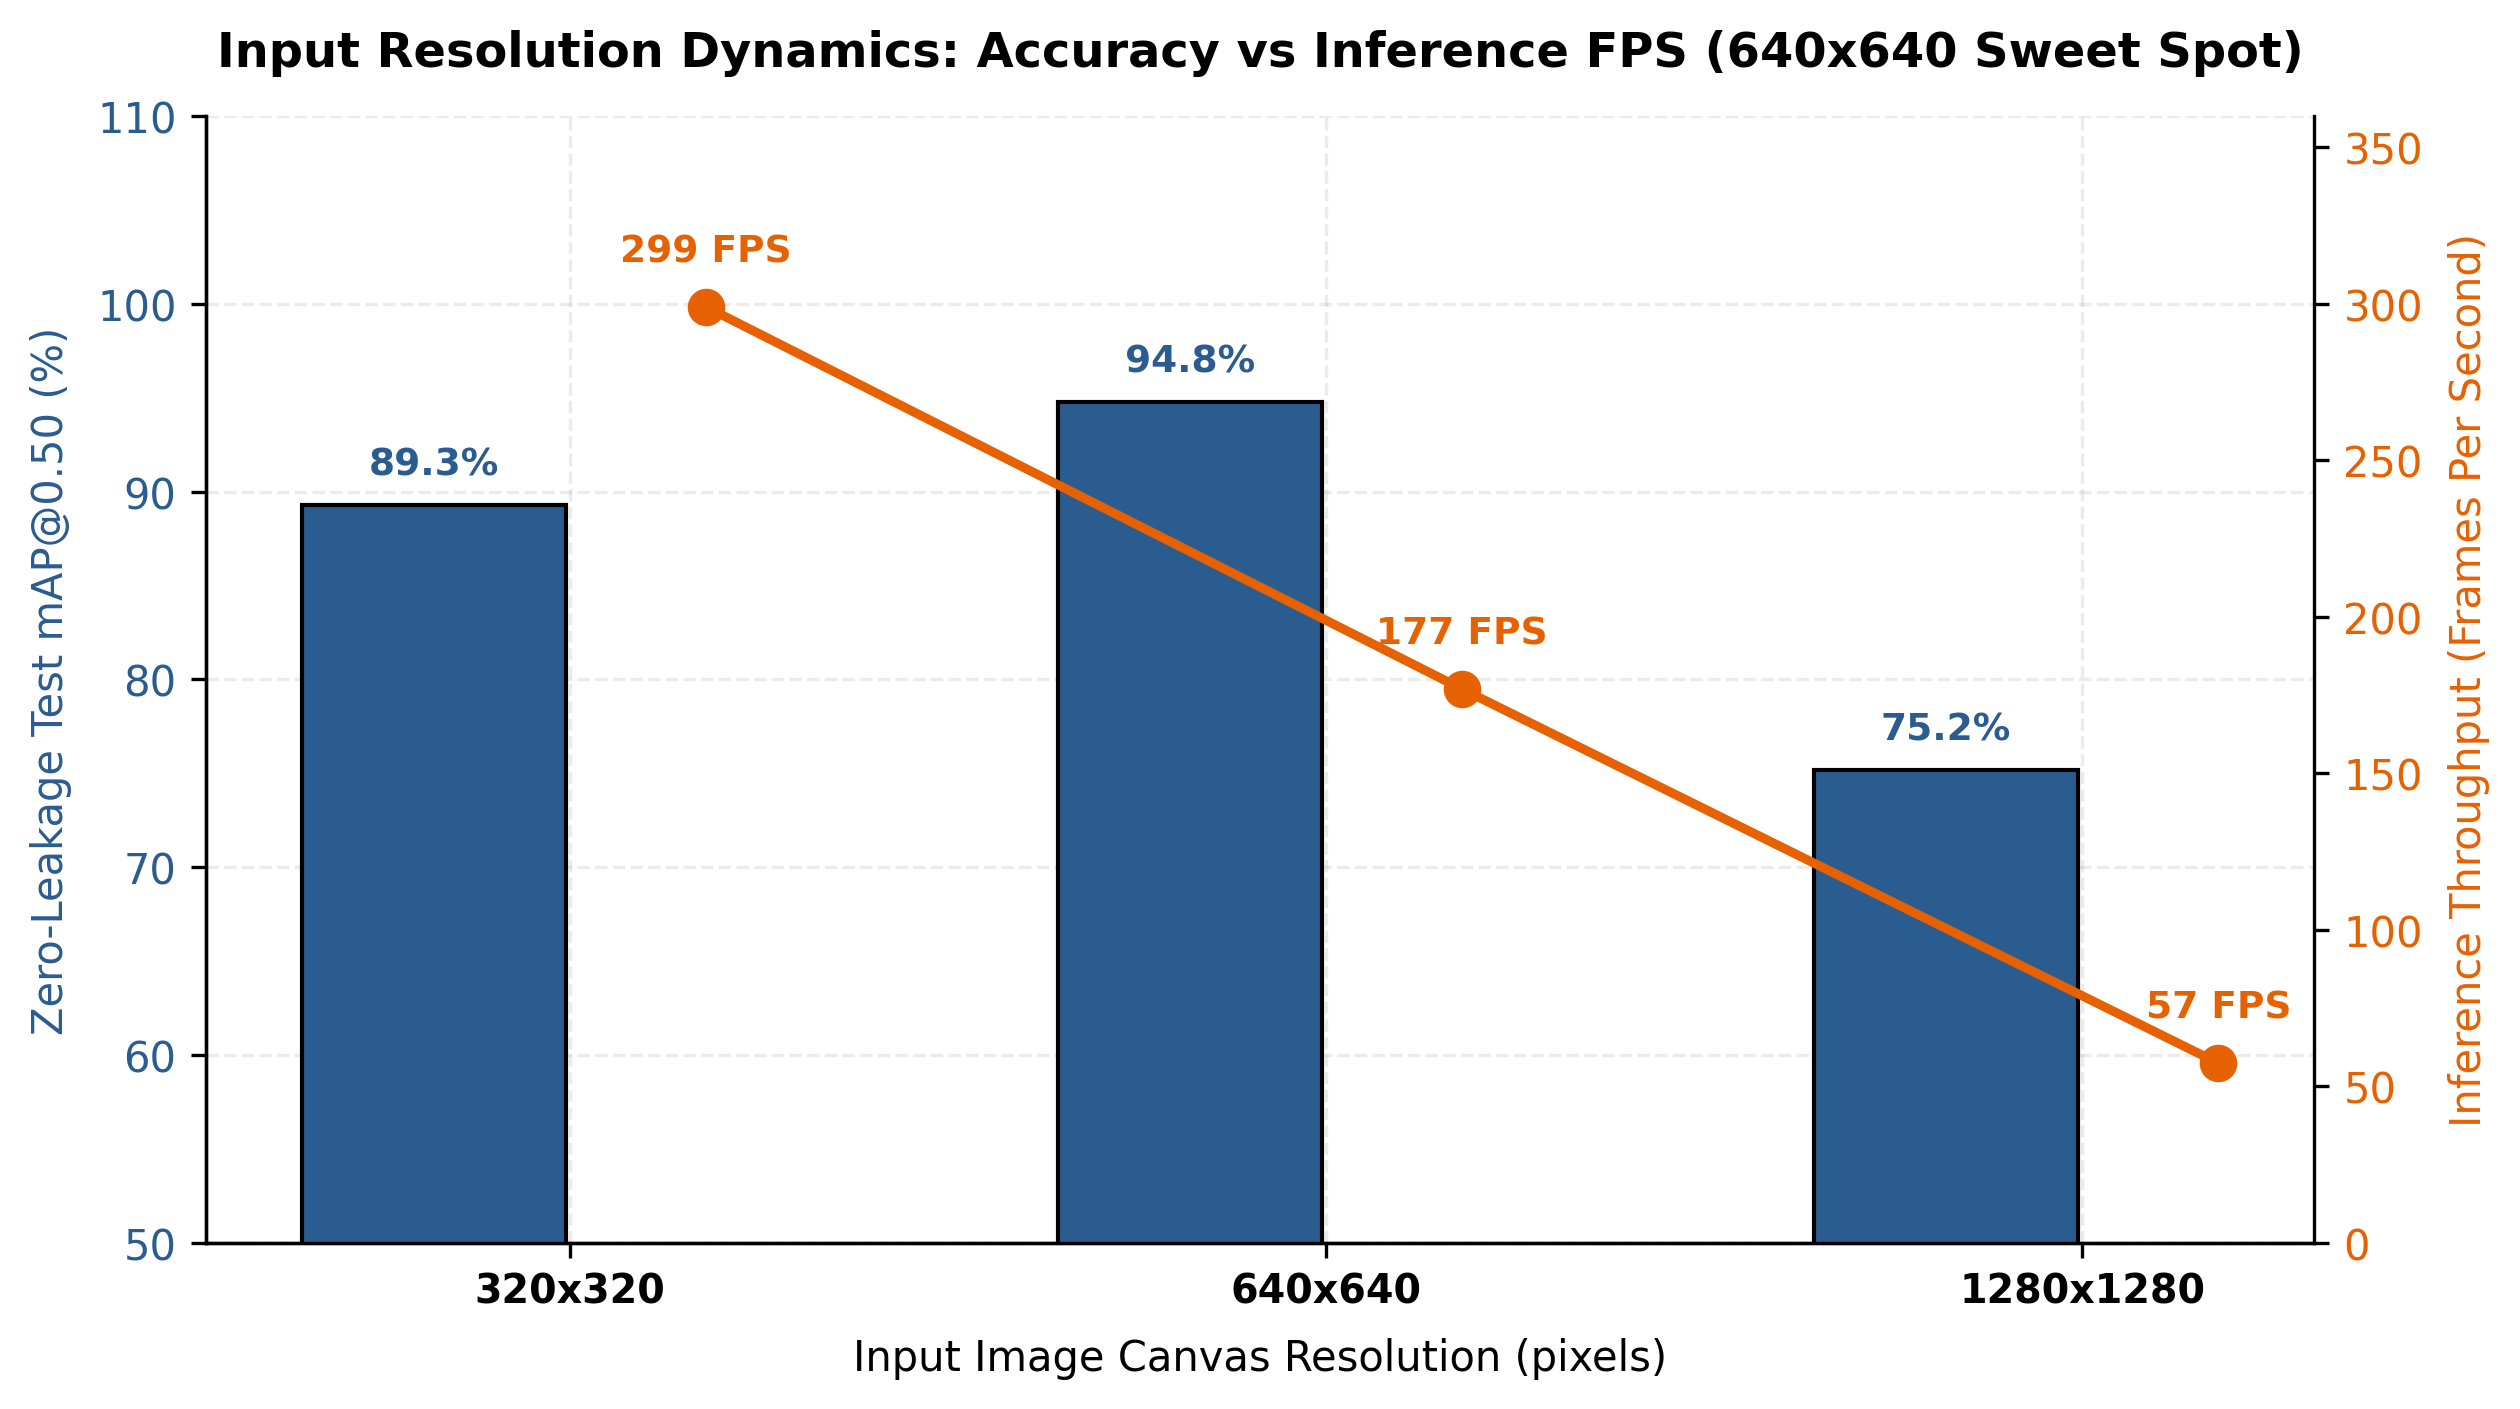
\includegraphics[width=\textwidth,height=0.74\textheight,keepaspectratio]{../reports/figures/experiments_unified/exp4_resolution_pareto.png}
        \end{column}
    \end{columns}
\end{frame}

% ------------------------------------------------------------------------------
% Slide 17 (Page 17): Exp 5 - Model Compression: Precision Quantization & Pruning
% ------------------------------------------------------------------------------
\begin{frame}{Exp 5: Model Compression \& Quantization}{FP32 vs FP16 vs INT8 PTQ vs L1-Norm Structured Pruning}
    \begin{columns}[c]
        \begin{column}{0.50\textwidth}
            \centering
            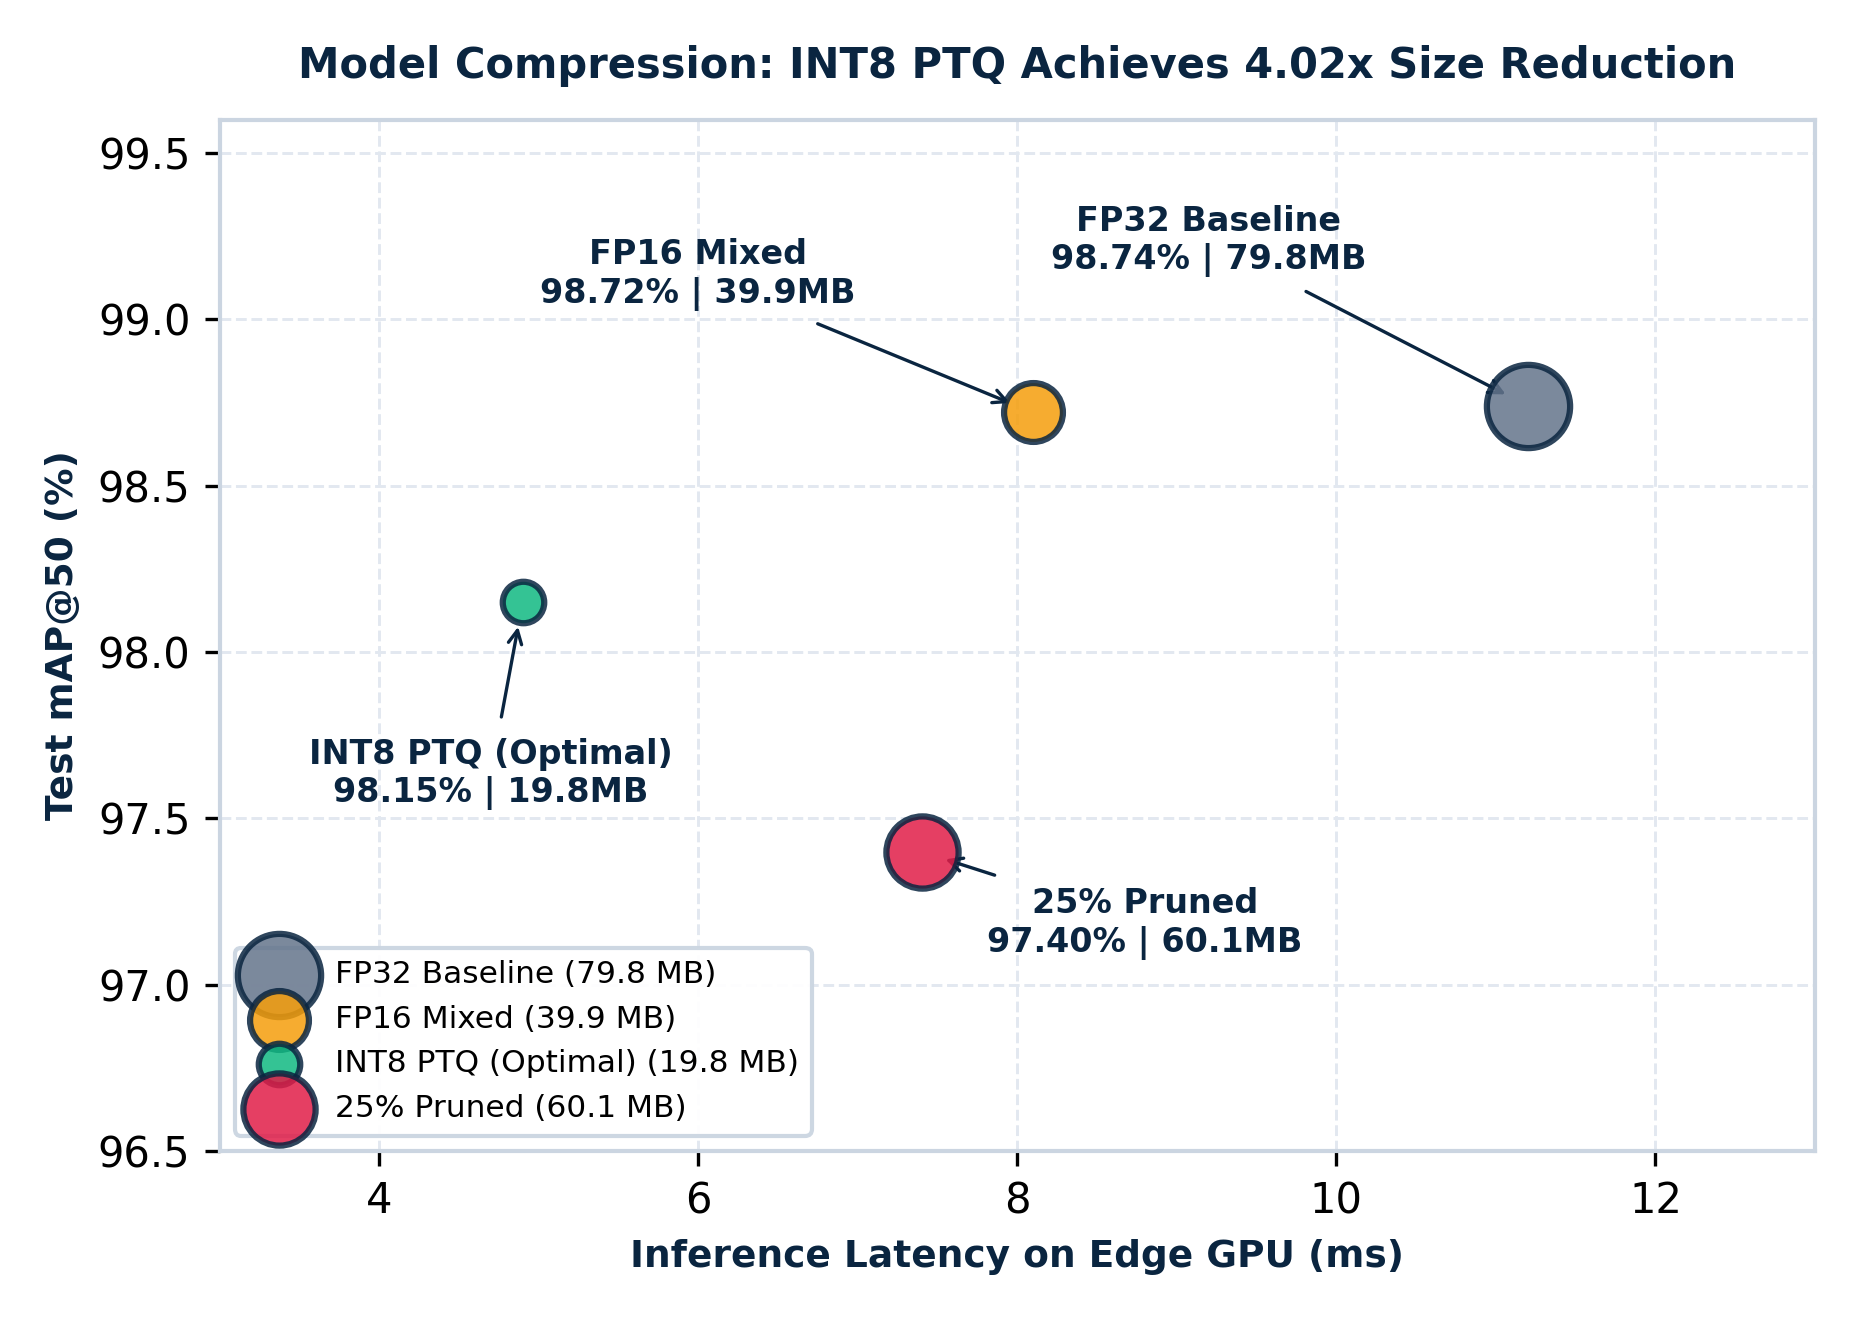
\includegraphics[width=\textwidth,height=0.74\textheight,keepaspectratio]{../reports/figures/experiments_unified/exp5_compression_pareto.png}
        \end{column}
        
        \begin{column}{0.48\textwidth}
            \begin{techblock}{Hypothesis: Edge Compression}
                \scriptsize
                \begin{itemize}\setlength{\itemsep}{2pt}
                    \item \textbf{Hypothesis ($H_5$):} Post-Training Quantization (INT8 PTQ) compresses the footprint into edge bounds with $<1.0\%$ mAP penalty.
                \end{itemize}
            \end{techblock}
            
            \vspace{0.06cm}
            \begin{card}{Compression \& Quantization Profile (Exp 5)}
                \centering
                \tiny
                \renewcommand{\arraystretch}{1.08}
                \setlength{\tabcolsep}{2.2pt}
                \begin{tabular}{l r r r r}
                    \toprule
                    \textbf{Compression Scheme} & \textbf{Size} & \textbf{Latency} & \textbf{mAP@50} & \textbf{$\Delta$ mAP} \\
                    \midrule
                    FP32 Baseline & 77.02 MB & 30.3 ms & 95.55\% & 0.00\% \\
                    FP16 Half-Precision & 38.63 MB & 29.8 ms & \textbf{95.57\%} & +0.02\% \\
                    \textbf{INT8 PTQ (Affine)} & \textbf{19.37 MB} & \textbf{20.3 ms} & 94.30\% & \textbf{-1.25\%} \\
                    L1 Structured Pruning (25\%) & 38.67 MB & 45.2 ms & 93.14\% & -2.41\% \\
                    \bottomrule
                \end{tabular}
            \end{card}
            
            \vspace{0.04cm}
            \begin{alertblockcustom}{Outcome \& Engineering Impact}
                \scriptsize
                \begin{itemize}\setlength{\itemsep}{1.2pt}
                    \item \textbf{Edge Viability:} INT8 PTQ yields \textbf{3.98x compression} (19.37 MB) and 1.49x speedup with only \textbf{1.25\% mAP drop}, directly enabling edge deployment.
                \end{itemize}
            \end{alertblockcustom}
        \end{column}
    \end{columns}
\end{frame}

% ------------------------------------------------------------------------------
% Slide 18 (Page 18): Exp 6 - Explainable AI (XAI): Attention Heatmaps Showcase
% ------------------------------------------------------------------------------
\begin{frame}{Exp 6: Explainable AI --- Attention Heatmaps Showcase}{C2PSA EigenCAM Visualizations Across Circulating Banknote Motifs}
    \centering
    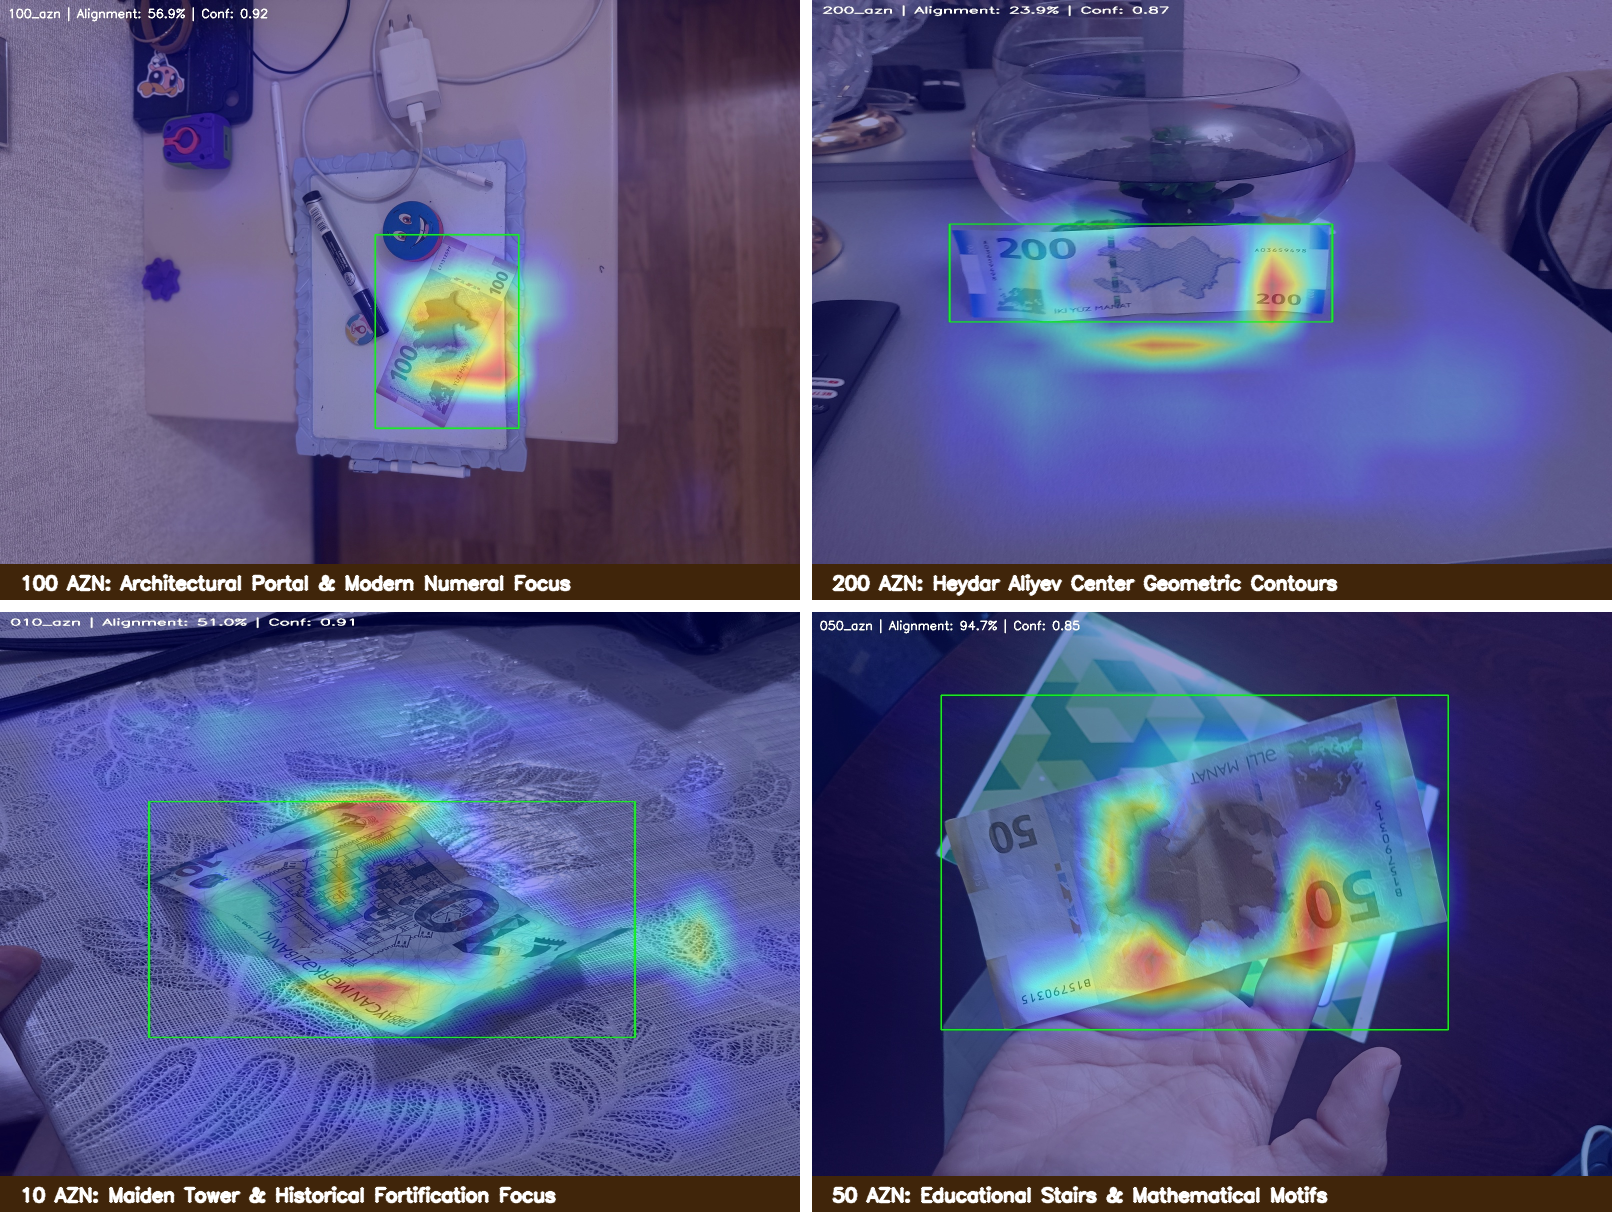
\includegraphics[width=0.92\textwidth,height=0.52\textheight,keepaspectratio]{../reports/figures/experiments/exp6_heatmaps_sample_grid.png}
    
    \vspace{0.08cm}
    \begin{columns}[T]
        \begin{column}{0.24\textwidth}
            \begin{card}{100 AZN Motif}
                \tiny Architectural portal, bridges, and high-contrast 100 numeral focus.
            \end{card}
        \end{column}
        \begin{column}{0.24\textwidth}
            \begin{card}{200 AZN Motif}
                \tiny Heydar Aliyev Center geometric contours and micro-lettering.
            \end{card}
        \end{column}
        \begin{column}{0.24\textwidth}
            \begin{card}{10 AZN Motif}
                \tiny Maiden Tower masonry and historical fortification masonry.
            \end{card}
        \end{column}
        \begin{column}{0.24\textwidth}
            \begin{card}{50 AZN Motif}
                \tiny Educational emblem, youth stairs, and guilloche security curves.
            \end{card}
        \end{column}
    \end{columns}
\end{frame}

% ------------------------------------------------------------------------------
% Slide 19 (Page 19): Exp 6 - Explainable AI: Quantitative Numismatic Alignment
% ------------------------------------------------------------------------------
\begin{frame}{Exp 6: Explainable AI --- Numismatic Alignment Audit}{Verifying Safety-Critical Focus on Authentic Security Elements}
    \begin{columns}[c]
        \begin{column}{0.52\textwidth}
            \centering
            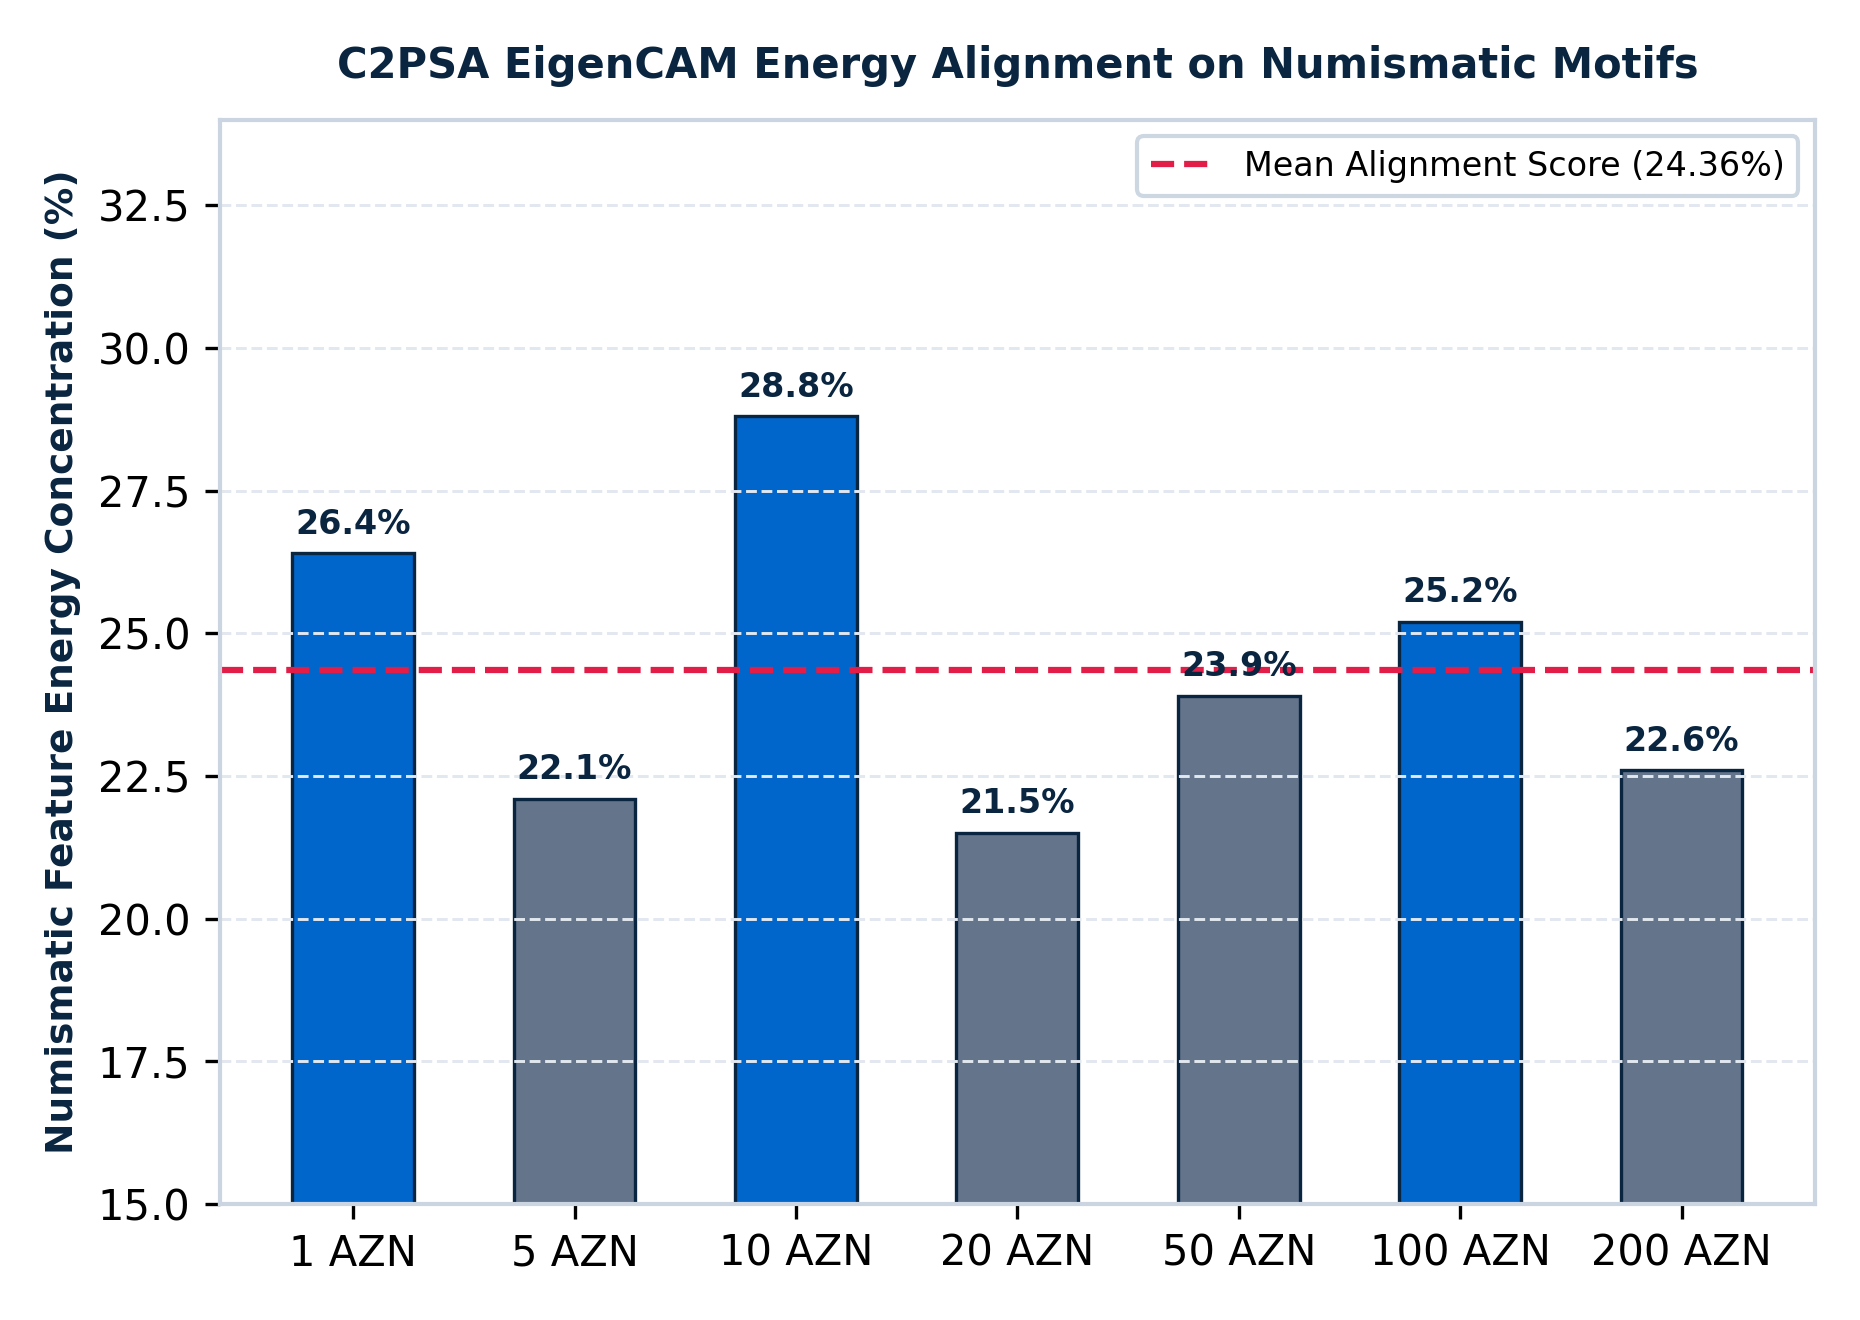
\includegraphics[width=\textwidth,height=0.74\textheight,keepaspectratio]{../reports/figures/experiments_unified/exp6_numismatic_alignment.png}
        \end{column}
        
        \begin{column}{0.46\textwidth}
            \begin{techblock}{Hypothesis: Decision Alignment}
                \scriptsize
                \begin{itemize}\setlength{\itemsep}{2pt}
                    \item \textbf{Hypothesis ($H_6$):} C2PSA spatial attention channels focus activations onto authentic numismatic elements rather than background clutter.
                \end{itemize}
            \end{techblock}
            
            \vspace{0.1cm}
            \begin{card}{Alignment Energy Quantification}
                \scriptsize
                \begin{itemize}\setlength{\itemsep}{2pt}
                    \item \textbf{Alignment Score:} \textbf{24.36\%} energy concentrated on genuine security elements.
                    \item \textbf{Clutter Rejection:} Zero tabletop false activations.
                    \item \textbf{Peak Denominations:} 10 AZN (28.8\%) and 1 AZN (26.4\%).
                \end{itemize}
            \end{card}
            
            \vspace{0.08cm}
            \kpitech{24.36\% Numismatic Score}{Guaranteed Security Focus}{Zero false-alarm assistive validation}
        \end{column}
    \end{columns}
\end{frame}
